The LES implemented at the Disaster Prevention Research Institute of Kyoto
University is a high-resolution simulator used to model turbulent flows in urban
environments. The LES does this by using mesoscale \footnote{Dimensions up to
several hundred kilometres} realistic meteorological simulations and Geographic
Information System (GIS) data to model the elevation, buildings, and other
objects in the environment. The LES has a number of different subroutines to
calculate different effects however the most important, and more computationally
intensive subroutine, is the Poisson equation solver. The solver uses successive
over-relaxation (SOR) to solve the linear system of equations. This calculates
the pressure of the air in the simulated area.

The LES is written in FORTRAN 77 and runs in a single thread. The main time step
loop has a number of sequential calls to subroutines that each have their own
distinct task over the three dimensional area under simulation:

\begin{itemize}[noitemsep,nolistsep]

    \item[velnw] updates the wind velocities

    \item[bondv1] calculates boundary conditions such as the initial wind
    profile, inflow, and outflow

    \item[velfg] calculates the body forces

    \item[feedbf] calculates the effects caused by the buildings in the area
    being modeled

    \item[les] calculates the viscosity terms using the Smagorinsky model.

    \item[adam] conducts the Adams-Bashforth time integration

    \item[press] solves the Poisson equation using SOR and is the most
    computationally intensive subroutine in the LES codebase with more than half
    of the runtime being spent in this subroutine during each time step.

\end{itemize}

\begin{figure}
    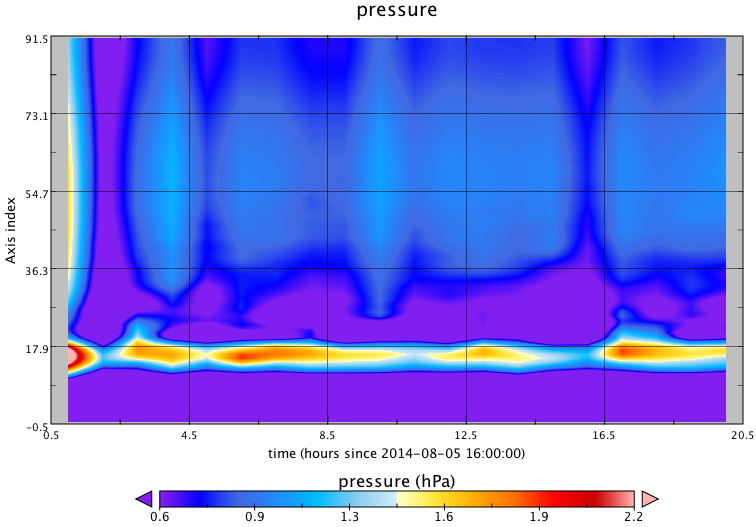
\includegraphics[width=0.5\textwidth]{graphs/pressure_in_LES_output_p.png}
    \caption{LES Pressure Output from Panoply}
    \label{fig:lespressure}
\end{figure}

Output is stored in the netCDF file format. This can then be fed into WRF or
another climate system or viewed visually. Figure~\ref{fig:lespressure} shows an
example output from the LES. The output shown is a two dimensional slice of
pressure. The output is a series of three dimensional grids over regular
intervals in the simulation. These grids are manually analysed for turbulent
flows, evidenced by the rate of change and shape of change in the colour code
pressure and velocity graphs.
